%! TEX root = ../000-main.tex
\chapter{Observed functional data and its computational representation}
\chaptermark{Observed FD}

\section{Observing functional data in practice}%
\sectionmark{Observing Functional Data}

It is not possible to observe (sample) and/or to record (store)
a functional data $\mathcal X_i$ for all $t\in T=[a,\,b]$:
\begin{itemize}
	\item The measurement devices are only able to sample the phenomenon
	      only at discrete instants (even if the sample frequency is extremely high).
	\item Given that $T = [a,\,b]$ is an infinite set, saving all
	      $\mathcal X_i$ for all $t\in T$ would imply to use an infinite amount of memory.
\end{itemize}

In practice, $\mathcal X_i$ is sampled/recorded in a finite grid:
\begin{equation*}
	t_{i1} < \cdots < t_{im_i} \subset T
\end{equation*}
where $m_i$ is the number of samples. If $m_i$ is large enough,
the maximum difference between two consecutive samples
$\max_j\left\{t_{ij} - t_{i(j+1)}\right\}$ is small.

\begin{recap}{}{}
    \begin{itemize}
        \item In practice a functional data $\mathcal X$ is not fully observed.
            It is impossible to observe $\mathcal X(t)$ for all $t\in T$.
        \item Only a finite amount of values $\mathcal X(t_j)$ can be observed
            and registered, $t_j \in [A,\,B],\,j\in\mathds N$.

        \item The set of observed values is called the \emph{sample grid}.
        \item Moreover, the observation process can be affected by an observational noise.
    \end{itemize}
\end{recap}

This presents 4 scenarios, as depicted in \cref{fig:observed-fd-scenarios}:
\begin{figure}[H]
	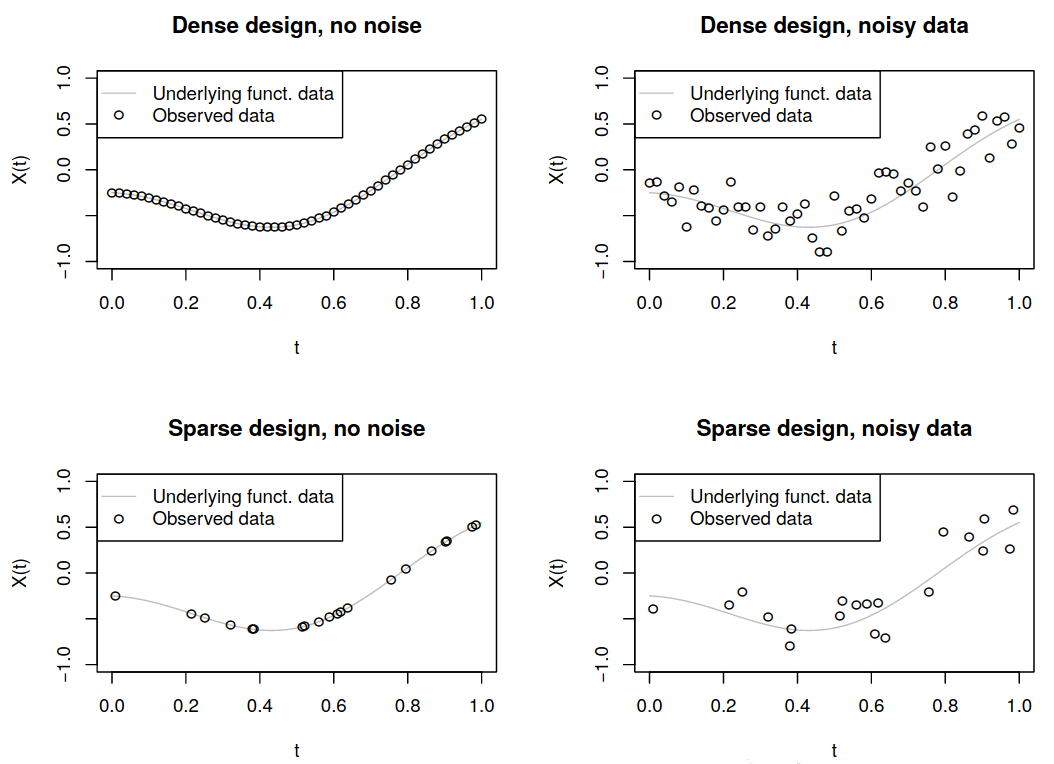
\includegraphics{observed-fd-scenarios}
	\caption{Example scenarios for the observation of functional data}
	\label{fig:observed-fd-scenarios}
\end{figure}

\subsection{Dense design}

\begin{definition}{Evenly Spaced Sampling}{}
	\begin{equation*}
		t_{j+1} - t_j = \delta = \frac{t_m - t_1}{m}
	\end{equation*}
\end{definition}

\subsection{Sparse design}

% TODO

\begin{definition}{Functional Data (practical definition)}{fdp}
	Multivariate data with an ordering on the dimensions.

	This definition implicitly assumes a common ordered design:
	\begin{equation*}
		t_1 < \cdots < t_m :  \mathcal X_i (t_j) + \varepsilon_{ij},\quad
		j=1,\ldots,m,\quad i=1,\ldots,n
	\end{equation*}
	\tcblower
	\begin{note}
		Ordering in the $m$ dimensions of the data is \emph{crucial},
		because it allows us to talk about \iemph{close dimensions}%
		\footnote{Close dimensions are more correlated than \iemph{distant dimensions}.}%
		.
	\end{note}
	\begin{note}
		This is an alternative way of saying that the functional data
		$\mathcal X_i$ are smooth functions.
	\end{note}
\end{definition}

\begin{question*}
	{Is FDA really different from Multivariate Analysis?}
	\begin{itemize}
		\item In Functional Data Analysis, the methods and procedures are
		      designed as if the functional data $\mathcal X_i(t),\,t\in T=[a,\,b]$
		      were available.
		\item Then the observed data $x_{ij}$ are used to estimate the required
		      elements.
		\item Finally, the outputs are displayed taking into account the functional
		      character of the objects of interest.
	\end{itemize}
\end{question*}



\pagebreak
\section[Representing functional data]{Representing functional data in a computer}

\subsection{Matrix representation}

\subsubsection{Common evenly spaced dense design}
Common evenly spaced (or not) dense design with no noisy data:
\begin{equation*}
	x_{ij} = \mathcal X_i(t_j),\quad j=1,\ldots,m,\quad i=1,\ldots,n
\end{equation*}
already have a good representation as a $n\times m$ matrix
$\boldsymbol X = \left(x_{ij}\right)_{n\times m}$.

If $\delta = t_{j+1} - t_j$ is small enough, many (if not all) the
required methods and procedures in FDA can be satisfactorily numerically
approximated using this matrix representation.

\subsubsection{Other situations}
For functional data with noisy data and/or sparse design, \iemph{smoothing
	methods} allows us to obtain a smooth estimation of the
underlying functional data with a common evenly spaced dense design. This
estimations can then be represented as a matrix.

\subsection{Basis-expansion representation}

Consider the square integrable Hilbert Space $L^2(T)$.
The inner product $\langle f, g\rangle = \int_T f(t)g(t)\,dt$ induces
a norm $\|f\| = \sqrt{\langle f, f\rangle}$ and a distance
between two functions $d(f, g)$:
\begin{equation*}
	d(f, g) = \lVert f - g \rVert = \sqrt{\langle f - g, f - g\rangle}
\end{equation*}

\begin{prop*}{}
	Any separable Hilbert space admits a countable orthonormal basis.
\end{prop*}

\begin{definition}{Countable Orthonormal basis}{}\index{countable orthonormal basis}\index{basis}

	A countable family $B = \{\phi_k\}_{k\in\mathds N},\, \phi_k\in{}H$ of functions
	that satisfies:
	\begin{alignat*}{2}
		\langle \phi_k, \phi_j\rangle        & = 0, \quad                                              & \forall & k,j \in \mathds N,\; k\neq j
		\tag{Orthogonality}                                                                                                                            \\
		\lVert \phi_k \rVert                 & = 1 \quad                                               & \forall & k \in \mathds N \tag{Normalization} \\[1em]
		\span\span\forall f\in L^2(T)\quad \exists \{c_k^f\}_{k\in\mathds N} \subset \mathds R \text{ s.t.}                                            \\
		\lim_{K\to\infty} \left\lVert
		f - \sum_{k=1}^{K} c_k^f \phi_k
		\right\rVert                         & = 0                                                                                                     \\
		\span\span\text{In fact, } c_k^f = \langle f,\, \phi_k\rangle                                                                                  \\
		f = \sum_{k=1}^{\infty} c_k^f \phi_k & = \sum_{k=1}^{\infty} \langle f,\, \phi_k\rangle \phi_k
		\tag{Completeness}
	\end{alignat*}
	\tcblower
	\begin{note}
		If $B$ satisfies only the last condition (\iemph{completeness}),
        it is called a basis of $L^2(T)$. (But it is not an \iemph{orthonormal basis})
	\end{note}
\end{definition}

\subsubsection{Finite basis-expansions for representing functional data}

For the orthonormal basis, when $K$ goes to infinity:
\begin{equation*}
    \lim_{K\to\infty} \left\lVert
    f - \sum_{k=1}^{K} c_k^f \phi_k
    \right\rVert \downarrow 0
\end{equation*}

Then the $K$-dimensional approximations (\iemph{finite basis-expansions})
\begin{equation*}
    f \approx = \sum_{k=1}^{K} \langle f,\, \phi_k\rangle \phi_k
\end{equation*}
are increasingly good approximations of $f$ as $K$ increases.

\begin{marker}
    Finite expansions in a given basis are a standard way to represent functional
    data.
\end{marker}

\subsubsection{Fourier basis}

A very convenient (before the computer age) example of
basis for the functional space $L^2(T),\,T=[a,\,b]$ is the \iemph{Fourier basis}:

\begin{definition}{Fourier Basis}{}\index{Fourier basis}
    Basis which elements are sine and cosine functions with
    increasing frequencies:
    \begin{align*}
        \text{Let } \omega = \frac{2\pi}{b-a}& \\
        B = \{&
            1/\sqrt{b-a},\\
              &\sqrt{2/(b-a)}\cos(\omega t),\,
            \sqrt{2/(b-a)}\sin(\omega t),\\
              &\ldots \\
              &\sqrt{2/(b-a)}\cos(\omega k t),\,
            \sqrt{2/(b-a)}\sin(\omega k t),\ldots\,
        \}
    \end{align*}
    \begin{note}
        \textbf{Inconvenient:} The representation of a function $f$ in $B$ is
        \emph{always} a periodic function in $T = [a,\,b]$, even if $f$ is not.
    \end{note}
    \begin{note}
        \iemph{B-spline bases} Are a non-orthogonal basis which are a
        good alternative to the Fourier basis. They consist of
        piecewise polynomials 
    \end{note}
\end{definition}

\section{Regularization in FDA}

\begin{definition}{Regularization}{}\index{regularization}
    Penalization of a function for \iemph{lack of smoothness}.
\end{definition}

In FDA, regularization is required in two different problems:
\begin{itemize}
    \item Transforming observed non-smooth data to functional smooth data.
    \item Estimating smooth functional parameters in functional models.
\end{itemize}

\subsection{Transforming observed data into functional smooth data}

Observed data:
\begin{equation*}
    x_{ij} = \mathcal X_i(t_j) + \varepsilon_{ij},\, j = 1,\ldots, m, i = 1,\ldots, n
\end{equation*}
$t_{j+1} - t_j = \delta = (t_m - t_1)/(m)$ with $m$ large.

$\varepsilon_{ij}$ are independent zero-mean random variables
(possibly with a common variance or even identically distributed).

Desired objects: $\mathcal X_i(t),\,t\in T = [a,\,b],\, i = 1,\ldots, n$.

More precisely, we want to have a computer valid representation of
$\mathcal X_i(t)$. One of:
\begin{itemize}
    \item \textbf{Matrix representation}
    \item \textbf{Basis-expansion representation}
\end{itemize}

Assume that a basis representation if desired using $\{\phi_k\}_{k=1,\ldots,K}$.

Let $\hat{\mathcal X}_i(t) = \sum_{k=1}^K c_{k}^{\mathcal X_i} \phi_k(t),\,t \in [a,\,b]$

The coefficients $c_1,\ldots,c_K$ are chosen as the solution of the problem:

\begin{problem}{}{}
    \begin{equation*}
        \min_{c_1,\ldots,c_K} 
        \sum_{j=1}^{n_j} \left(
            x_{ij} - \hat{\mathcal X}_i(t_{ij})
        \right)^2
        + \lambda
        \int_{a}^{b} \left(
            L(\mathcal X_i)(t)
        \right)^2\, dt
    \end{equation*}
    where $L$ is a \iemph{linear differential operator} (e.g. a derivative):
    $L(f) = \sum_{h=1}^H a_h f^{(h)}$.
\end{problem}

Penalization $L(f) = f^{(2)}$ is called \emph{second-order smoothing} and
is used to avoid \emph{oscillations} in the approximations (bumpy functions),
since:
\begin{equation*}
    \int_{a}^{b} \left(
        f^{(2)}(t)
    \right)^2\, dt
\end{equation*}
is a measure of the \iemph{total curvature} of the function $f$.

\begin{note}
    This penalization is associated with cubic splines bases (as we will show later).
\end{note}

\subsubsection{Estimating functional parameters}

In most cases, estimating a (regression) model for functional data
consists of finding a function (the model parameter is a whole function)

The estimation problem has an expression of this kind:
\begin{problem}{}{}
    \begin{equation*}
        \min_{f:[a,\,b] \to \mathds R} T(f; \mathcal X_1,\ldots,\mathcal X_n)
    \end{equation*}
\end{problem}

This is an infinite-dimensional problem (very difficult) and moreover,
there is no guarantee that the estimated functional parameter is a smooth 
function.

A feasible option is to look for the best parameter belonging to the space of functions spanned by
a finite subset of a basis of functions.

Then the problem becomes a finite-dimensional optimization problem.

In addition to that, a regularization term is added to the objective function
in order to have a smooth solution

Let $f(t) = \sum_{k=1}^K \beta_k B_k(t),\,t\in [a,\,b]$
The coefficients $\beta_k$ are chosen as the solution of the problem:
\begin{problem}{}{}
    \begin{equation*}
        \min_{\beta_1,\ldots,\beta_K} T(f; \mathcal X_1,\ldots,\mathcal X_n)
        + \underbrace{\lambda_T \int_{a}^{b} \left(
            L(f)(t)
    \right)^2\, dt}_{\text{regularization term}}
    \end{equation*}
where $\lambda_T$ is a \iemph{smoothing parameter}.
\end{problem}

\begin{note}
When estimating functional parameters, finite basis expansion is
the functional representation of choice.
\end{note}

% \section{Developments in bases of functions}
% \section{Smoothing: Kernel, Local Polynomials, Splines}
% \section{Registration and transformations of functional data}

\section[Registration of functional data]{Registration of functional data (or time warping)}

Variability among functional data:
\begin{itemize}
    \item \textbf{Variability in amplitude} (values of the functions)
    \item \textbf{Variability in phase} (argument of the functions)
\end{itemize}

\begin{example}{Variability in amplitude}{} Human growth functions

    Every person has its own biological clock, that does not always coincide 
    with what the calendar marks. Some children get the growth
    spurt before another.
\end{example}

\begin{example}{Variability in phase}{} Temperature data

    In some areas winters arrive earlier than in others. Some years the summer is ahead and
    others are late.
\end{example}

\begin{definition}{Warping functions}{}\index{warping functions}
    increasing functions with $h_i(a) = a$ and $h_i(b) = b$ that are
    able to synchronize functions so that they do not
    present \iemph{phase variability}.
\end{definition}

\begin{definition}{Registration}{}\index{registration}
    (or \emph{time warping})

    Any technique to estimate the warping functions $h_i$ with the aim of \emph{reducing
    the variability in phase} among functions.

    \tcblower
    \begin{itemize}
        \item Shifting the argument of each function by a different quantity.
        \item Aligning several \emph{key points} (or \emph{marks}) at all the functions.
        \item Looking for generic warping functions $h_i$ in a non-parametric way, trying to
            minimize a global measure of variability in phase among the functions.
    \end{itemize}
\end{definition}

\begin{figure}[H]
    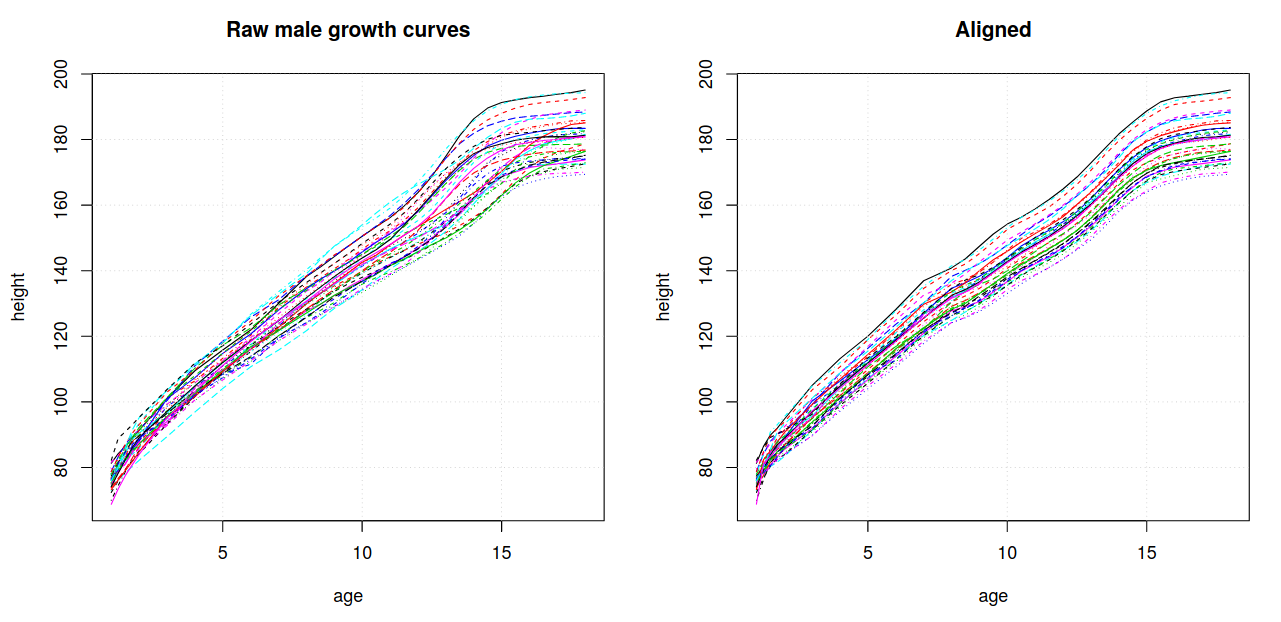
\includegraphics{male_growth_alignment}
    \caption{Registration of growth curves}
\end{figure}
